\subsubsection{Codificaci\'on e implementaci\'on de algoritmo en el robot en la primera iteraci\'on 2}
    La implementaci\'on en el robot no cambia respecto a c\'omo se
        estuvo planeando desde el inicio, debido a que las rutas son
        obtenidas de acuerdo con la simulaci\'on del Physarum, que,
        una vez finalizada esta, a partir de una serie de condiciones y
        convirtiendo el camino en coordenadas las cuales el robot
        pueda interpretar para realizar su recorrido de la mejor forma
        posible, se pueda llegar de un punto inicial a un punto final
        de forma correcta.
        \vskip 0.5cm
    Como se planteo desde el inicio, el algoritmo debe generar
        su ruta con ayuda del Physarum, y a partir de esta, generar
        una serie de coordenadas las cuales el robot pueda seguir
        para moverse de un punto al otro. En la implementaci\'on, el
        archivo generado a partir de la ruta que se obtuvo con el
        Physarum, se puede ver en la Figura \ref{fig:Archivoderutas01}.
    \vskip 0.5cm
    %imagen
    \begin{figure}[htbp]
        \centering
        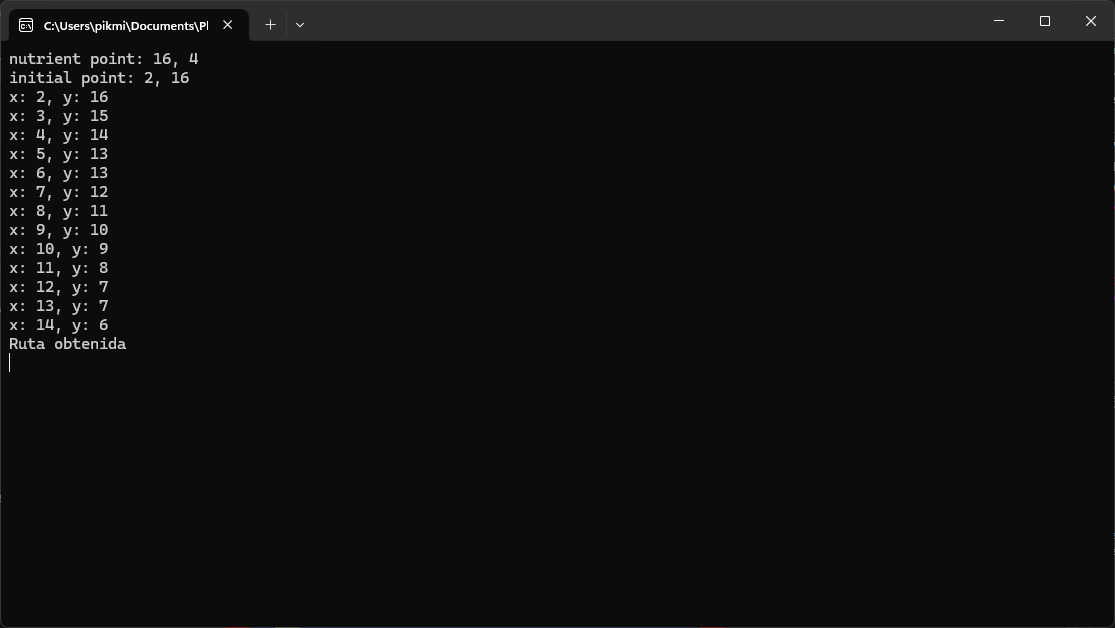
\includegraphics[width=0.5\textwidth]{./images/Pruebas/simulador/image043.png}
        \caption{Archivo de rutas}
        \label{fig:Archivoderutas01}
    \end{figure}
    \vskip 0.5cm
    Las coordenadas est\'an dadas de acuerdo con el punto de
        partida, que est\'a representado a partir del punto inicial en el
        simulador, hasta el destino, el cual es uno de los nutrientes
        en el simulador del Physarum y son de vital importancia para
        poder generar la ruta, ya que, con la ausencia de estos, no se
        puede generar una ruta. Las coordenadas est\'an ordenadas deforma de aparici\'on, lo que hace que haya una forma de
        seguirla correctamente y no se deba de perder, o seguir la
        ruta de manera err\'onea.